\documentclass[a4paper, 11pt, fleqn, normalem]{report}

\usepackage{../../LaTeX-Templates/Notes}

\titleformat{\chapter}{\fontsize{13}{15}\bfseries\normalfont}{\textbf{}}{1em}{}
\setcounter{tocdepth}{1}
\setcounter{secnumdepth}{1}

\title{Foundations of Physics Year 1 \\ Modern Physics \vspace{-20pt}}
\author{Stewart Clark}
\date{\vspace{-15pt}Epiphany Term 2017}
\rhead{\hyperlink{page.1}{Go to TOC}}

\begin{document}

\maketitle
\thispagestyle{fancy}

\tableofcontents

\chapter{Relativity}
\section{Classical Relativity}
A reference frame can be considered to be a set of axes with an observer at the origin \\
The observer is stationary in their own reference frame \\
In an inertial frame of reference, the observer does experience a net force (ignore gravity for now) \\
Inertial reference frames move at constant velocity with respect to each other \\
There is no unique reference frame; none are any more special than another - although, careful choice of reference frame can make problems simpler \\
In inertial reference frames, the laws of physics are the same -- through experimental observation \\
Use dash (') to denote reference frames e.g. O, O', O'' \\
This is not a derivative \\
We won't use $f'(x)$ to denote derivative, instead will use Leibniz's $\frac{df}{dx}$

\section{Transforms}
Galilean transforms between two intertial points will tell us how the co-ordinates of a point (x, y, z, t) in O will be seen by O' i.e. (x', y', z', t')

\section{Velocities}
In an inertial frame, O, let's assume there is an object moving with velocity ($v_{x}$, $v_{y}$, $v_{z}$) \\
Now let's have another observer, O', moving at velocity ($u_{x}$, $u_{y}$, $u_{z}$) with respect to O \\
Then:
\begin{itemize}
    \item[] $v_{x}' = v_{x} - u_{x}$
    \item[] $v_{y}' = v_{y} - u_{y}$
    \item[] $v_{z}' = v_{z} - u_{z}$
\end{itemize}
\textbf{Example:} Align system aling common x--x' axis \\
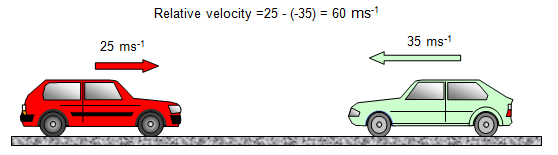
\includegraphics{Cars.png} \\
In O, we know that:
\begin{gather*}
    u_{x} = -35\text{mph},~~~v_{x} = 25\text{mph}
\end{gather*}
Want $v_{x}'$ (speed of car coming from left relative to green car):
\begin{gather*}
    v_{x}' = v_{x} - u_{x} \\
    ~~~    = 25 - (-35) \\
    ~~~    = 60\text{ms}^{-1}
\end{gather*}
We can show that Newton II is invariant:
\begin{gather*}
    a_{x} = \frac{dv_{x}}{dt} = \frac{d(v_{x}' + u_{x})}{dt'}\cdot \frac{dt'}{dt} = a_{x}' + 0 \\
    \underline{a_{x} = a_{x}'}
\end{gather*}

\section{Position Transforms}
Sync clocks: $t = t' = 0$ when O' passes O \\
After a time $t = t'$,  the origings will be a distance vt apart \\
Therefore we get:
\begin{itemize}
    \item[] $x = x' + vt$
    \item[] $y = y'$
    \item[] $z = z'$
\end{itemize}
Or:
\begin{itemize}
    \item[] $x' = x - vt$
    \item[] $y' = y$
    \item[] $z' = z$
\end{itemize}
Note that:
\begin{gather*}
    v_{x} = \frac{dx}{dt} = \frac{d}{dt'}(x' + vt)\cdot\frac{dt'}{dt} \\
    v_{x} = v_{x}' + v
\end{gather*}

\section{Special Relativity}
Spaceship at $v = 1000\text{ms}^{-1}$; shoots missile at $v' = 2000\text{ms}^{-1}$; to external observer, $v' = 3000\text{ms}^{-1}$ \\
But what if it fires a laser? \\
Laser travels at speed of light so observer sees laser at $c + 1000\text{ms}^{-1}$ \\
This contradicts experiment \\
No matter how we measure c in a vacuum, we always get the same value \\
Experimentally, c is constant/invariant

\section{Postulates}
\begin{enumerate}
    \item Speed of light is a constant, independent of reference frame
    \item Laws of physics are independent of reference frame
\end{enumerate}

\section{Thought Experiment}
We are observers on Earth (inertial frame of reference) \\
A spaceship travels past the Earth at speed, u \\
We have two inertial frames: Earth, O, \& spaceship, O' \\
$O \xrightarrow{u} O'$ \\
On the spaceship, someone does the following: \\
A light source fires a pulse of light across the spaceship, it hits a mirror on the other side of the spaceship and returns to the source \\
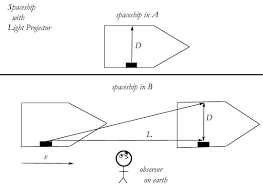
\includegraphics{Gamma.png} \\
$\Delta t' = \frac{2D}{c}$

O ref -- time $\Delta t$ \\
In time $\Delta t$, spaceship travels distance $L = u\Delta t$ \\
Path length in O is $2\sqrt{d^{2} + (\frac{u\Delta t}{2})^{2}}$ \\
Time taken, $\Delta t = \dfrac{2\sqrt{d^{2} + (\frac{u\Delta t}{2})^{2}}}{2}$
\begin{gather*}
    d = \frac{c}{2}\Delta t' \implies \\
    \Delta t = \frac{2}{c}\sqrt{(\frac{c\Delta t'}{2})^{2} + (\frac{u\Delta t}{2})^{2}} \implies \\
    \Delta t^{2} = \Delta t'^{2} + \frac{u^{2}}{c^{2}}\Delta t^{2} \implies \\
    \Delta t^{2}\Big(1 - \frac{u^{2}}{c^{2}}\Big) = \Delta t'^{2} \implies \\
    \Delta t = \frac{\Delta t'}{\sqrt{1 - \tfrac{u^{2}}{c^{2}}}}
\end{gather*}
Define $\gamma$:
\begin{gather*}
    \gamma = \frac{1}{\sqrt{1 - \tfrac{u^{2}}{c^{2}}}} \implies \\
    \Delta t = \gamma\Delta t'
\end{gather*}
Look at $\gamma$ as a function of $\beta = \frac{u^{2}}{c^{2}}$: \\
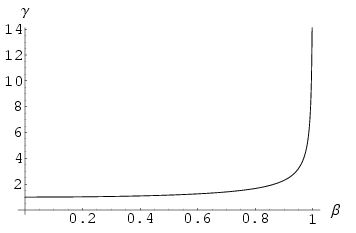
\includegraphics{Gammafn.jpg} \\
$\implies \Delta t > \Delta t'$ \\
Clocks moving at some speed with respect to us appear to be going slower \\
Let $u = 300\text{ms}^{-1}$ \\
Then:
\begin{equation*}
    \gamma(300) = \frac{1}{\sqrt{1 - (\tfrac{300}{3\times10^{8}})^{2}}} \approx 1\times10^{-12}
\end{equation*}

\section{Simultaneity}
Let's let an event be observed by O at (x, y, z, t) \& by O' at (x', y', z', t') \\
When we say something is simultaneous, we mean we observe it at the same time \\
So if $t = t'$, then they agree it is simultaneous \\
Also note in above derivation we had two events: light leaving source and light returning \\
In O', let the events be at: \\
($x_{1}'$, $y_{1}'$, $z_{1}'$, $t_{1}'$) \& ($x_{2}'$, $y_{2}'$, $z_{2}'$, $t_{2}'$) \\
Defined $\Delta t' = t_{2}' - t_{1}'$ \\
But we had $x_{1}' = x_{2}'$ etc.

\textbf{Example:} Cosmic rays from space interact with atoms in atmosphere to create muons at speed $v = 0.99c$, with a lifetime of $1.56\times10^{-5}s$ \\
In the muon's reference frame, how long does it exist? \\
$\Delta t'$ -- lifetime in muon's reference frame \\
$\Delta t$ -- time in our frame
\begin{gather*}
    \gamma(0.99c) = \frac{1}{\sqrt{1 - 0.99^{2}}} \approx 7.1 \\
    \Delta t = \gamma\Delta t' \implies \\
    \Delta t' = \frac{\Delta t}{\gamma} \approx 2.2\times10^{-6}s
\end{gather*}

\section{Length}
Spaceship, O' $\rightarrow$ u \\
Earth, O \\
A -- pulse of light emitted from source in the direction of travel and travels a distance l' \\
B -- reflects off mirror and travels back along same path \\
2l' travelled in time $\Delta t' \therefore 2l' = c\Delta t'$:
\begin{gather*}
    (1)~~l + u\Delta t_{1} = c\Delta t_{1} \\
    ~~~~~\Delta t_{1} = \frac{l}{c - u} \text{ [half experiment]} \\
    (2)~~l - u\Delta t_{2} = c\Delta t_{2} \\
    ~~~~~\Delta t_{2} = \frac{l}{c + u}
\end{gather*}
Whole experiment:
\begin{gather*}
    c\Delta t = c\Delta t_{1} + c\Delta t_{2} \\
    ~~~~~ = \frac{cl}{c - u} + \frac{cl}{c + u} \\
    ~~~~~ = \frac{2c^{2}l}{c^{2} - u^{2}} \\
    ~~~~~ = \frac{2l}{1 - \tfrac{u^{2}}{c^{2}}} \\
    ~~~~~ = 2l\gamma^{2} \\
    c\Delta t = c\gamma\Delta t' \\
    l\gamma = l'
\end{gather*}

\section{Frame-Invariant Quantities}
c is invariant but are there others?
\begin{gather*}
    \text{(Interval)}^{2} = \text{(c}\times\text{separation in time)}^{2} - \text{(spacial separation)}^{2} \\
    \Delta s^{2} = (c\Delta t)^{2} - (\Delta x)^{2} - (\Delta y)^{2} - (\Delta z)^{2}\text{ is invariant}
\end{gather*}

\section{Proper Time \& Length}
t' \& l' -- defined within stationary reference frame
\begin{gather*}
    t = \gamma t' \\
    l = \frac{l'}{\gamma}
\end{gather*}
l' is the longest distance and t' is the shortest time

\section{Lorentz Transforms}
So for only specific cases: \\
In O, let a point, P, in space-time be (x, y, z, t) \\
Let O', be a frame moving at speed u with respect to O along their common x-x' axis \\
The Point P in O' is seen at (x', y', z', t') \\
How are these related? \\
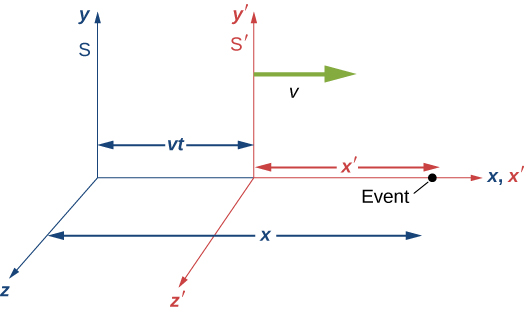
\includegraphics{Axes.jpg} \\
If we let $t = t' = 0$ as O' passes O \\
Considering x-coordinate of point, P:
\begin{gather*}
    x = ut + [x']' = ut + \frac{x'}{\gamma} \\
    x' = \gamma [x - ut]
\end{gather*}
Repeat for O': $x = \gamma [x' + ut']$
Rearrange this for x'
\begin{gather*}
    x' = -ut' + \frac{x}{\gamma} \\
    \gamma(x - ut) = ut' + \frac{x}{\gamma} \\
    t' = \gamma(t - \frac{ux}{c^{2}})
\end{gather*}
There is no relative motion in the y- or z-directions:
\begin{gather*}
    y' = y \\
    z' = z
\end{gather*}
If we are looking for length, this is the difference in two coordinates, and similar for time period
\begin{gather*}
    L = x_{2} - x_{1} \\
    L' = x_{2}' - x_{1}' \\
    ~~~ = \gamma(x_{2} - ut_{2}) - \gamma(x_{1} - ut_{1}) \\
    ~~~ = \gamma[(x_{2} - x_{1}) - u(t_{2} - t_{1})] \\
    ~~~ = \gamma[\Delta x - u\Delta t]
\end{gather*}
This takes away the simultaneity of measurements \\
The same thing can be done for time:
\begin{gather*}
    \Delta t = t_{2} - t_{1} \\
    \Delta t' = t_{2}' -t_{1}' \\
    ~~~~\, = \gamma(t_{2} - \frac{ux_{2}}{c^{2}}) - \gamma(t_{1} - \frac{ux_{1}}{c^{2}}) \\
    ~~~~\, = \gamma[(t_{2} - t_{1}) - \frac{u}{c^{2}}(x_{2} - x_{1})] \\
    ~~~~\, = \gamma[\Delta t - \frac{u}{c^{2}}\Delta x]
\end{gather*}
\textbf{Example:} Train enters tunnel of length 56m at a speed of $\frac{45}{53}c$ \\
Define:
\begin{itemize}
    \item[] Event A as end of train entering tunnel
    \item[] Event B as front of train leaving tunnel
\end{itemize}
Observer at entrance says both events are simultaneous \\
2nd observer on rear of train sees things differently \\
If event A happens at $t = t' = 0$, when does observer on train see event B? \\
How long is the train? \\
Firstly, get gamma:
\begin{gather*}
    \gamma = \frac{1}{\sqrt{1 - \tfrac{u^{2}}{c^{2}}}} \\
    \gamma = \frac{1}{\sqrt{1 - (\tfrac{45}{53})^{2}}} = \frac{53}{28} \\
    x_{B}' - x_{A}' = \frac{53}{28}[(x_{B} - x_{A}) - \frac{45}{53}c(t_{B} - t_{A})] \\
    t_{B}' - t_{A}' = \frac{53}{28}\Big[(t_{B} - t_{A}) - \frac{45}{53c}\Big] \\
    \implies x_{B}' -x_{A}' = 106\text{m -- proper length of train} \\
    \implies t_{B}' - t_{A}' \approx -0.3\mu\text{s -- on the train}
\end{gather*}
The negative time difference implies that B happens before A in that time frame

\section{Velocities}
\vspace{-24pt}
\begin{gather*}
    x' = \gamma(x - ut) \\
    t' = \gamma\Big(t - \frac{ux}{c^{2}}\Big)
\end{gather*}
Take time derivative of position to get velocity:
\begin{gather*}
    v_{x}' = \frac{dx'}{dt'} = \frac{dx'}{dt}\cdot\frac{dt}{dt'} = \frac{dx'}{dt}\Big/\frac{dt'}{dt} = \frac{\tfrac{dx}{dt} - u}{1 - \tfrac{u}{c^{2}}\cdot\tfrac{dx}{dt}} \\
    v_{x}' = \frac{v_{x} - u}{1 - \tfrac{u}{c^{2}}v_{x}} \\
    v_{y}' = \frac{dy'}{dt'} = \frac{dy'}{dt}\cdot\frac{dt}{dt'} = \frac{dy'}{dt}\Big/\frac{dt'}{dt} = \frac{\tfrac{dy}{dt}}{\gamma(1 - \tfrac{u}{c^{2}}\cdot\tfrac{dx}{dt})} \\
    v_{y}' = \frac{v_{y}}{\gamma(1 - \tfrac{u}{c^{2}}v_{x})}
\end{gather*}

\section{Coordinate Transforms Summary}
\vspace{-24pt}
\begin{gather*}
    x' = \gamma(x - ut) \\
    y' = y \\
    z' = z \\
    t' = \gamma(t - \frac{ux}{c})
\end{gather*}

\section{Velocity Transforms Summary}
\vspace{-24pt}
\begin{gather*}
    v_{x}' = \frac{v_{x} - u}{1 - \tfrac{u}{c^{2}}v_{x}} \\
    v_{y}' = \frac{v_{y}}{\gamma(1 - \tfrac{u}{c^{2}}v_{x})} \\
    v_{z}' = \frac{v_{z}}{\gamma(1 - \tfrac{u}{c^{2}}v_{x})}
\end{gather*}

\textbf{Example: }Two cars travelling towards each other at 0.6c according to an observer at the side of the road \\
How fast does one car see the other approaching? \\
Observer by road -- O \& Car -- O' \\
$u = 0.6c$ \& $v_{x} = -0.6c$
\begin{gather*}
    v_{x}' = \frac{v_{x} - u}{1 - \tfrac{uv_{x}}{c^{2}}} \\
    ~~~ = \frac{-0.6c - 0.6c}{1 + \tfrac{0.6c\times0.6c}{c^{2}}} \\
    ~~~ = -\frac{1.2c}{1.36} = -0.88c
\end{gather*}

\textbf{Example: }Two spaceships of proper length 100m travelling towards each other at 0.8c to external observer \\
How long is spaceship?
\begin{gather*}
    \gamma = \frac{1}{\sqrt{1 - (\tfrac{0.8c}{c})^{2}}} = \frac{5}{3} \\
    l = \frac{l'}{\gamma} = \frac{100\times3}{5} = 60\text{m}
\end{gather*}
How fast do the ships see each other?
\begin{gather*}
    v_{x} = -0.8c,~~~u = 0.8c \\
    v_{x}' = \frac{-0.8c - 0.8c}{1 + (\tfrac{0.8c}{c})^{2}} = \frac{-1.6c}{1.64} \approx -0.975
\end{gather*}
How long does one ship measure the other to be?
\begin{gather*}
    \gamma = \frac{1}{\sqrt{1 - (\tfrac{0.975c}{c})^{2}}} \approx 4.56 \\
    \implies l = \frac{100}{4.56} = 21.9
\end{gather*}

\section{Relativistic Momentum}
Classically, $\underline{p} = m\underline{v}$ is considered: \\
Consider snooker balls colliding -- \\
\textbf{Ball A}
\begin{gather*}
    v_{Ax} = 0 \implies v_{Ax}' = \frac{v_{Ax} - u}{1 - \tfrac{v_{Ax}u}{c^{2}}} = -u \\
    v_{Ay} = ? \implies v_{Ay}' = \frac{v_{Ay}}{\gamma}
\end{gather*}
\textbf{Ball B}
\begin{gather*}
    v_{Bx}' = 0 \implies v_{Bx} = \frac{v_{Bx}' + u}{1 + \tfrac{v_{Bx}'u}{c^{2}}} = u \\
    v_{By}' \implies v_{By} = \frac{v_{By}'}{\gamma(1 + \tfrac{v_{Bx}'u}{c^{2}})} = \frac{v_{By}'}{\gamma}
\end{gather*}
Factor of $\frac{1}{\gamma}$ in velocites which will break conservation of momentum \\
$\gamma \rightarrow 1$ as $u \rightarrow 0$ so relativistic alteration still tends to classical equation above \\
Let's define $\underline{p} = \gamma m\underline{v}$ as conserved momentum
\begin{equation*}
    \underline{p} = (\gamma m_{0})\underline{v}
\end{equation*}
$m_{0}$ is defined as the rest mass of an object:
\begin{equation*}
    m = \gamma m_{0}
\end{equation*}

\section{Relativistic Force}
\vspace{-24pt}
\begin{gather*}
    \underline{F} = \frac{d\underline{p}}{dt} \\
    \underline{F} = \frac{d}{dt}\frac{m_{0}\underline{v}}{\sqrt{1 - (\tfrac{v}{c})^{2}}}
\end{gather*}
Consider F parallel to v:
\begin{gather*}
    \underline{F} = \gamma m_{0}\frac{d\underline{v}}{dt} + m_{0}\underline{v}\frac{d\gamma}{dt} \\
    ~~ = \gamma m_{0}\frac{d\underline{v}}{dt} + m_{0}\underline{v}\frac{d\gamma}{d\underline{v}}\cdot\frac{d\underline{v}}{dt}
\end{gather*}
Evaluate $\frac{d\gamma}{d\underline{v}}$:
\begin{gather*}
    \frac{d\gamma}{d\underline{v}} = \frac{d}{d\underline{v}}\Big(\frac{1}{\sqrt{1 - (\tfrac{v}{c})^{2}}}\Big) = \frac{v}{c^{2}}\frac{1}{(1 - (\tfrac{v}{c})^{2})^{3/2}} = \frac{v}{c^{2}}\gamma^{3} \\
    \underline{F} = \gamma m_{0}\underline{a} + m_{0}\Big(\frac{v}{c}\Big)\gamma^{3}\underline{a} \\
    \text{Use substitution: }\gamma = \frac{1}{\sqrt{1 - (\tfrac{v}{c})^{2}}} \implies \frac{v^{2}}{c^{2}} = 1 - \frac{1}{\gamma^{2}} \\
    \rightarrow \underline{F} = \gamma m_{0}\underline{a} + m_{0}\Big(1 - \frac{1}{\gamma^{2}}\Big)\gamma^{3}\underline{a} \\
    \therefore \underline{F} = m_{0}\gamma^{3}\underline{a}
\end{gather*}
Let's look at F perpendicular to v i.e. circular motion \\
v is constant so $\frac{d\gamma}{dt} = 0$ \\
So from above, the second term is zero
\begin{gather*}
    \therefore \underline{F} = \gamma m_{0}\underline{a}
\end{gather*}

\section{Relativistic Energy}
For F parallel to v:
\begin{gather*}
    W = \int_{0}^{x} F\,dx = \int_{0}^{x} \gamma^{3} m_{0}a\,dx \\
    a\,dx = \frac{dv}{dt}\,dx = dv\,\frac{dx}{dt} = v\,dv \\
    W = \int_{0}^{v} m_{0}\gamma^{3}v\,dv = m_{0}\int_{0}^{v} \frac{1}{(1 - (\tfrac{v}{c})^{2})^{3/2}}v\,dv \\
    \text{Substitution: }\alpha = \frac{v^{2}}{c^{2}} \implies v^{2} = c^{2}\alpha \implies 2v\,dv = c^{2}\,d\alpha \\
    W = m_{0}c^{2}\int_{0}^{(\tfrac{v}{c})^{2}} \frac{d\alpha}{2(1 - \alpha)^{3/2}} \\
    ~~~ = m_{0}c^{2}\Big(\frac{1}{\sqrt{1 - \alpha}}\Big)\Bigg|_{0}^{(\tfrac{v}{c})^{2}} \\
    W = m_{0}c^{2}(\gamma - 1) \\
    KE = m_{0}c^{2}(\gamma - 1)
\end{gather*}
Look for classical result: $v = 0 \implies KE = 0$ \\
Note:
\begin{gather*}
    \text{Since }(1 + x)^{n} = 1 + nx + n(n - 1)\frac{x^{2}}{2} + \cdots,\\
    \text{then }\gamma = \frac{1}{\sqrt{1 - (\tfrac{v}{c})^{2}}} \implies 1 + \frac{v^{2}}{2c^{2}} + \frac{3v^{4}}{8c^{4}} + \cdots
\end{gather*}
Thus, when $v << c$, we have:
\begin{equation*}
    KE  = m_{0}c^{2}\Big[\Big(1 + \frac{v^{2}}{2c^{2}}\Big) - 1\Big] = \frac{1}{2}m_{0}v^{2}
\end{equation*}
KE appears to have two parts:
\begin{equation*}
    KE = m_{0}c^{2}(\gamma - 1) = \gamma m_{0}c^{2} - m_{0}c^{2}
\end{equation*}
The first part depends on v, but the second only on m \\
This gives us a clue! \\
This is telling us that an object with a mass $m_{0}$, has an "intrinsic" energy of:
\begin{equation*}
    E = m_{0}c^{2}
\end{equation*}
Let us define the total energy of an object as KE + intrinsic energy:
\begin{gather*}
    E = \gamma m_{0}c^{2},~~[m = \gamma m_{0}] \\
    \underline{E = mc^{2}}
\end{gather*}
In all of our equations, $\gamma$ was there, hence v. We now have equations of energy and momentum which need v so let's eliminate v:
\begin{gather*}
    \text{Energy -- }\gamma = \frac{E}{m_{0}c^{2}} \implies \frac{E^{2}}{m_{0}^{2}c^{4}} = \frac{1}{1 - (\tfrac{v}{c})^{2}} \\
    \text{Momentum -- }\gamma = \frac{p}{m_{0}c} \implies \frac{p^{2}}{m_{0}^{2}c^{2}} = \frac{1}{1 - (\tfrac{v}{c})^{2}} \\
    \therefore E^{2} = (m_{0}c^{2})^{2} + (pc)^{2}
\end{gather*}

\section{Relativistic Transforms Summary}
\vspace{-22pt}
\begin{gather*}
    m = \gamma m_{0}~~~~~F = \gamma^{3}ma\,(||) \\
    \underline{p} = \gamma m\underline{v}~~~~~F = \gamma ma\,(\perp) \\
    E^{2} = (m_{0}c^{2})^{2} + (pc)^{2}
\end{gather*}
\textbf{Example: }An oil tanker of 100kT travels at 0.3ms$^{-1}$ \\
How fast must a 1g bird go to have the same momentum?
\begin{gather*}
    p_{\text{tank}} = 10^{8}\times0.3 = 3\times10^{7}\text{ kg ms}^{-1}\\
    p_{\text{bird}} = \gamma m_{0}v = 3\times10^{7}\text{ -- solve for v:} \\
    v = 0.99995c
\end{gather*}
\textbf{Example: }A rocket has rest mass of 1 T \\
Its engine produces a thrust of 50 kN \\
What is the acceleration from rest and what is the acceleration when the rocket is at 0.99c?
\begin{gather*}
    \text{Rest -- }\gamma = 1 \implies a = \frac{F}{m} = \frac{50000}{1\times10^{3}} = 50\text{ms}^{-2} \\
    v = 0.99c~\therefore~\gamma = \frac{1}{\sqrt{1 - 0.99^{2}}} \approx 7 \\
    F || v ~\therefore~ a = \frac{F}{m\gamma^{3}} = \frac{50\times10^{3}}{10^{3}\times343} = 0.15\text{ms}^{-2}
\end{gather*}
\textbf{Example: }A particle of rest mass $1\frac{MeV}{c^{2}}$ and KE of 2 MeV collides with a stationary particle of rest mass $2\frac{MeV}{c^{2}}$ \\
Units -- Usually mass is kg, energy J \\
Often express energies in terms of electron volts, eV: $1\;eV = 1.6\times10^{-19}\;J \implies 1\;MeV = 1.6\times10^{-13}\;J$ \\
For mass, we can use $m = \frac{E}{c^{2}}$ \\
a) What is the totaly energy of the system?
\begin{gather*}
    P1:~E_{1} = 2\,MeV + 1\,MeV = 3\,MeV \\
    P2:~E_{2} = 2\,MeV \\
    \text{Total: }E_{1} + E_{2} = 5\,MeV
\end{gather*}
b) What is the speed of the first particle before collision?
\begin{gather*}
    3\,MeV = \gamma m_{0}c^{2} = \gamma(1\frac{MeV}{c^{2}})c^{2} = \gamma\cdot1\,MeV \\
    \implies \gamma = 3 \rightarrow v = \sqrt{\frac{8}{9}}c
\end{gather*}
c) What is the initial momentum of the system?
\begin{gather*}
    E^{2} = p^{2}c^{2} + (m_{0}c^{2})^{2} \\
    \implies p = \sqrt{8}\,\frac{MeV}{c}
\end{gather*}

\section{4-Vectors (not examinable)}
Returning to coordinate transforms, we have:
\begin{gather*}
    t' = \gamma\Big(t - \frac{ux}{c^{2}}\Big) \\
    x' = \gamma\Big(x - ut) \\
    y' = y \\
    z' = z
\end{gather*}
If we take a simple transform of a coordinate (x, y) rotated around the origin by an angle $\theta$, then we know:
\begin{equation*}
    \begin{pmatrix}
        x' \\
        y'
    \end{pmatrix}
    =
    \begin{pmatrix}
        \cos{\theta}  & \sin{\theta} \\
        -\sin{\theta} & \cos{\theta}
    \end{pmatrix}
\end{equation*}
Rearrange 1: $ct' = \gamma ct - \frac{\gamma u}{c}x$ \\
Rearrange 2: $x' = -\frac{\gamma u}{c}(tc) + \gamma x$
\begin{equation*}
    \begin{pmatrix}
        ct' \\
        x'  \\
        y'  \\
        z'
    \end{pmatrix}
    =
    \begin{pmatrix}
        \gamma             & -\frac{u\gamma}{c} & 0 & 0 \\
        -\frac{u\gamma}{c} & \gamma             & 0 & 0 \\
        0                  & 0                  & 1 & 0 \\
        0                  & 0                  & 0 & 1
    \end{pmatrix}
    \begin{pmatrix}
        ct \\
        x  \\
        y  \\
        z
    \end{pmatrix}
\end{equation*}
This is the Lorentz transform in matrix form \\
Consider $2\times2$ upper left matrix:
\begin{equation*}
    \begin{pmatrix}
        \gamma             & -\frac{u\gamma}{c} \\
        -\frac{u\gamma}{c} & \gamma
    \end{pmatrix}
\end{equation*}
Now look at its eigenvalues and plot them against $\frac{u}{c}$: \\
One value starts at one and tends to infinity as $\frac{u}{c}$ approaches one -- this is time dilation \\
The other also starts at one but tends to zero as $\frac{u}{c}$ approaches one -- this is length contraction \\
Let u be some reasonable speed, then our $2\times2$ transform does this:\\
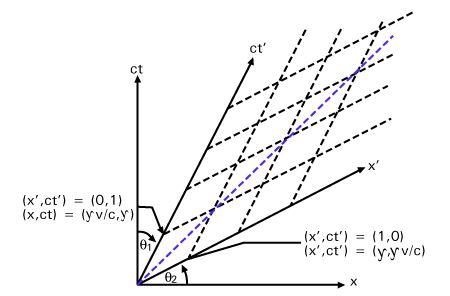
\includegraphics{Lorentz.jpg}

\chapter{Quantum Mechanics}
By the 1900s, physics was:
\begin{itemize}
    \item Mechanics (Newton)
    \item Gravity (Newton)
    \item Electricity and Magnetism (Maxwell)
    \item Thermodynamics (Kelvin)
    \item Statistical Physics
\end{itemize}
With this, we were able to describe almost all known physical phenomena at the time \\
There were some peculiarities and questions that were not yet answered but it was thought that they would be eventually by using the known laws\\
We had particles which obeyed Newton's laws and waves which obeyed Maxwell's equations

\section{Maxwell's Equations}
\begin{enumerate}
    \item Coulomb's Law -- force between charged particles
    \item Biot-Savart Law -- force between currents
    \item Faraday's Law -- changing magnetic field leads to a current
    \item Ampere's Law -- changing current leads to magnetic field
\end{enumerate}
What could we not answer?
\begin{itemize}
    \item What caused materials to emit light when heated?
    \item Why did the hot materials have a specific spectrum?
    \item Why does the sun shine for a long time?
    \item Why do some materials conduct electricity and some do not?
\end{itemize}

\section{Photoelectric Effect}
When light shines on a metal surface, if the frequency is high enough then:
\begin{enumerate}
    \item A current is observed, even in dim light
    \item KE of emitted electrons depends only on frequency
    \item No current if frequency of light is below a certain value
    \item For a given frequency, current increases with intensity
\end{enumerate}
This is a problem: it does not obey the wave nature of light \\
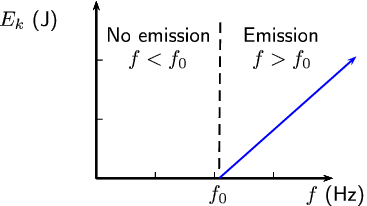
\includegraphics[scale=0.7]{Photoelec.png} \\
This $f_{0}$ is independent of intensity -- intensity just increases the number of electrons emitted, but not their energy \\
Let's put a voltage across the system: \\
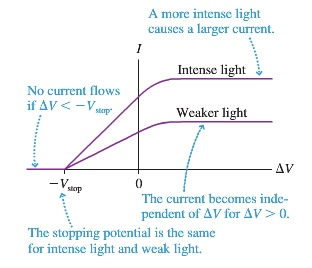
\includegraphics{currentvsvoltage.jpg} \\
We can explain this if light were made of particles, photons \\
Each particle has energy proportional to frequency
\begin{equation*}
    E \propto f
\end{equation*}
The constant of proportionality is Planck's constant, h
\begin{equation*}
    E = hf
\end{equation*}
The photoelectric effect tells us that light can behave as particles

It appears that there is some energy required to eject the electron and then the rest of the energy is transfered to KE \\
This initial energy for emission is material-dependent and is called "the work function"
\begin{equation*}
    E = hf - \phi,~~~[\phi\text{ is the work function}]
\end{equation*}
There is a threshold frequency, $f_{0}$ at which an electron is released with zero KE -- $\phi = hf_{0}$ \\
So note that if $hf < \phi$, since we cannot have negative KE, the photon is simply absorbed by the material and the material converts its energy into heat

\textbf{Example: }If light has wavelength 300nm (UV), incident onto a potassium surface \\
Electrons are emitted with maximum KE of 2.03 eV \\
(i) What is the energy of the photon?
\begin{equation*}
    E = hf = \frac{hc}{\lambda} = 4.13\,eV
\end{equation*}
(ii) What is the work function of the metal?
\begin{equation*}
    \phi = E - KE = 4.13 - 2.03 = 2.10\,eV
\end{equation*}
(iii) What is the maximum KE emitted electrons if light has $\lambda = 430$nm?
\begin{equation*}
    KE = \frac{hc}{\lambda} - \phi = 0.78\,eV
\end{equation*}
(iv) What is the threshold wavelength, $\lambda_{0}$ for potassium?
\begin{equation*}
    KE = 0 = \frac{hc}{\lambda_{0}} - \phi \implies \lambda_{0} = \frac{hc}{\phi} = 590\text{nm}
\end{equation*}

\section{Inverse Photoelectric Effect}
Can electrons emit photons? Do an experiment \\
If we use high-energy electrons, the following is obtained:

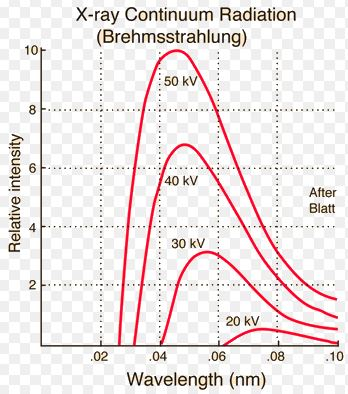
\includegraphics{Bremstrah.jpg}

This is called Brehmsstrahlung Radiation \\
The same equation is valid as for photoelectric effect

\textbf{Example: }Photon travels towards electron at rest, they collide and travel off at angles to the axis of original travel \\
Energy conservation:
\begin{gather*}
    pc + m_{0}c^{2} = p'c + E_{ea} \\
    E_{e}^{2} = (p_{p}c - p_{p}' + m_{0}c^{2})^{2} \\
    (m_{0}c^{2})^{2} + (p_{e}c)^{2} = (p_{p}c - p_{p}'c + m_{0}c^{2})^{2}
\end{gather*}
Momentum conservation:
\begin{gather*}
    p_{p} = p_{p}' + p_{e} \\
    p_{e} = p_{p} - p_{p}' \\
    p_{e}^{2} = p^{2} - p'^{2} - 2pp'\cos{\phi} \\
    \frac{m_{0}c}{p'} - \frac{m_{0}c}{p} = 1 - \cos{\phi} \\
    \frac{h}{p'} - \frac{h}{p} = \frac{h}{m_{0}c}(1 - \cos{\phi}) \\
    \lambda' - \lambda = \frac{h}{m_{0}c}(1 - \cos{\phi})\text{ -- Compton Scattering}
\end{gather*}

\section{Wave-Particle Duality}
Let's fire electrons through some slits (often thought of as particles):
\begin{figure}[H]
    \begin{subfigure}{0.6\textwidth}
        \caption{Classically expected result}
        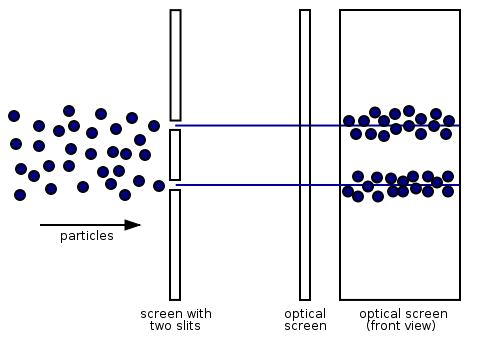
\includegraphics[width=\textwidth]{ClassicalDouble.png}
    \end{subfigure}

    \begin{subfigure}{0.8\textwidth}
        \caption{This is the actual result, with an interference pattern}
        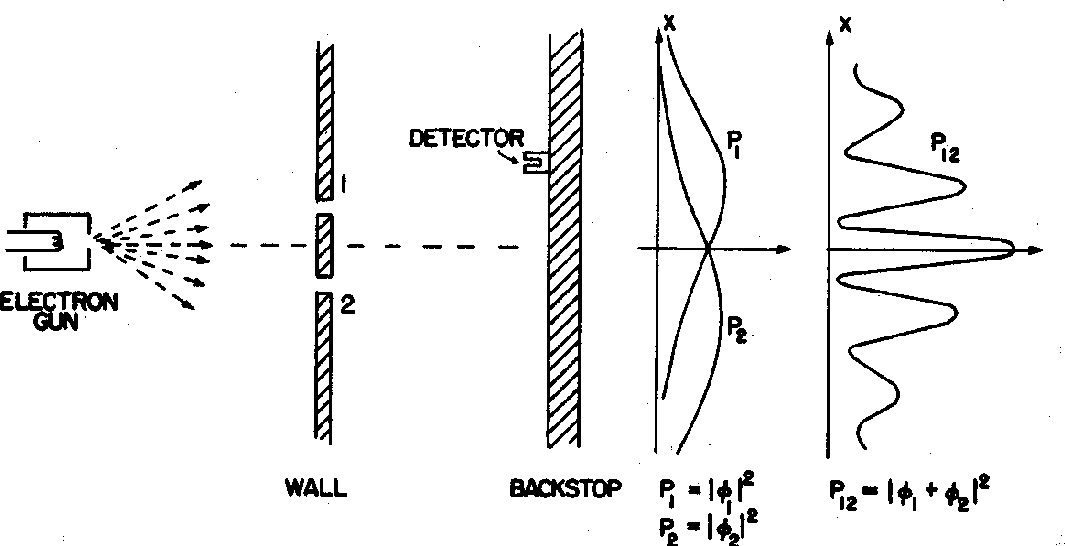
\includegraphics[width=\textwidth]{ActualDouble.png}
    \end{subfigure}
\end{figure}
What happens if we decrease the intensity of incoming particles to only one at a time? \\
Then if we measure to find location of the particle, it appears on the screen following the wave-like pattern where it indicates the probability of finding the particle at a particular position

\section{Heisenberg's Uncertainty Principle}
(proof later) \\
If there is uncertainty in the position of a particle, $\Delta x$, then the uncertainty in momentum, $\Delta p$, is related by:
\begin{equation*}
    \Delta x\,\Delta p \geq \frac{\hbar}{2},~~~\hbar = \frac{h}{2\pi}
\end{equation*}
This is not a criticism on the accuracy of ability to perform experiments; it is a fundamental statement about nature itself \\
(Proof later) -- this can be rewritten as:
\begin{equation*}
    \Delta E\,\Delta t \geq \frac{\hbar}{2}
\end{equation*}
\textbf{Example: }Estimate the size of a H-atom
\begin{gather*}
    \text{About }10^{-10}\text{m} = \text{\r{A}, the \r{A}ngstrom} \\
    E = \frac{p^{2}}{2m} - \frac{e^{2}}{(4\pi\epsilon_{0})r}
\end{gather*}
We don't know where the electron is so let $\Delta x \approx r$
Heisenberg gives us:
\begin{gather*}
    \Delta p \approx \frac{\hbar}{\Delta x} \approx \frac{\hbar}{r} \\
    E = \frac{1}{2m}\Big(\frac{\hbar}{r}\Big)^{2} - \frac{1}{4\pi\epsilon_{0}}\frac{e^{2}}{r}
\end{gather*}
Electron will be in a state that minimises energy so need:
\begin{gather*}
    \frac{dE}{dr} = 0 = -\frac{\hbar^{2}}{m}\frac{1}{r^{3}} + \frac{1}{4\pi\epsilon_{0}}\frac{e^{2}}{r^{2}} \\
    r = \frac{4\pi\epsilon_{0}\hbar^{2}}{me^{2}}
\end{gather*}
\textbf{Example: }Suppose that forces are mediated by the emission of a particle, if travelling some distance then being absorbed \\
If this is the process that binds nucleons, then how heavy is the particle?
\begin{equation*}
    \text{Use }\Delta E\,\Delta t \approx \hbar
\end{equation*}
If particle is moving quickly, let $E \approx mc^{2}$ and if is confined to nucleus, $R \approx 1.4\times10^{-15}$m hence
\begin{gather*}
    \Delta t \approx \frac{\hbar}{\Delta E} \approx \frac{\hbar}{mc^{2}} \\
    R \approx c\Delta t \approx \frac{c\hbar}{mc^{2}} \\
    \implies m = 140\,MeV
\end{gather*}
This is the prediction for a pion

\section{Particles and Waves}
\begin{tabular}{c|c|c}
              & Classical Physics    & Quantum Physics \\
    \hline
    Matter    & (particles) E, p     & (waves) $\lambda = \frac{h}{p}$, $f = \frac{E}{h}$                    \\
    \hline
    Radiation & (waves) f, $\lambda$ & (particles) $p = \frac{h}{\lambda}$, $E = hf$
\end{tabular} \\
The wave-particle duality model was mainly due to deBroglie \\
He suggested the symmetry between particles and waves and that they were interchangeable

\textbf{Example: }Electron accelerated to a KE of 10\,eV \\
What is the "deBroglie wavelength"? \\
\emph{Check for relativistic effects} (It's not)
\begin{equation*}
    \lambda = \frac{h}{p} = \frac{h}{\sqrt{2mE}} = \cdots = 0.39\,\text{nm}~(3.9\,\text{\r{A}})
\end{equation*}
Electrons at about this energy have a deBroglie wavelength of about that of inter-atomic spacing \\
In 1927, Davisson and Germer used electrons to diffract through a crystal \\
Similar to that of classical waves:
\begin{equation*}
    d\sin{\theta} = m\lambda
\end{equation*}
\textbf{Example: }Electrons with a KE of 54\,eV (non-relativistic) produces the first peak in a diffraction pattern at $\theta = 50\degree$ \\
(1) Get wavelength: $\lambda = \frac{h}{p} = \cdots = 0.167$nm \\
(2) If the interatomic spacing is $d = 0.215$mm, check result:
\begin{gather*}
    m\lambda = d\sin{\theta} = \cdots = 0.165\text{nm}
\end{gather*}
\textbf{Example: }What is the deBroglie wavelength of a particle with KE of 1\,eV, 1\,keV, 1\,MeV, 1\,GeV? \\
(i) 1\,eV $\rightarrow 1.23$nm \\
(ii) 1\,keV $\rightarrow 0.039$nm [non-relativistic] \\
(iii) 1\,MeV $\rightarrow E = KE + m_{0}c^{2}$, also $E^{2} = (pc)^{2} + (m_{0}c^{2})^{2}$
\begin{gather*}
    \implies p^{2} + \frac{(KE + m_{0}c^{2})^{2}}{c^{2}} - \frac{(m_{0}c{2})^{2}}{c^{2}} \\
    \implies \lambda = \frac{h}{p} = 0.87\text{pm}
\end{gather*}

\section{Particles Behaving Like Waves}
What is the physics that governs the equation of a wave? \\
We want to know about the wave equation to solve to get the wave function \\
This function is usually given the symbol, $\Psi$ \\
Similar to waves, the intensity of this is $|\Psi(x,\:t)|^{2}$ \\
We will soon see this will give us the probability of finding a particle at a certain location at a certain time \\
(Actually $|\Psi(x,\:t)|^{2}\,dx\,dt$ is probability function in $x \rightarrow x + dx,~~t \rightarrow t + dt$) \\
Equation governing this is known as \underline{Schr\"{o}dinger's Equation}

\section{Atomic Spectra}
In the late 1800s, experiments were done that determined the individual colours of light that was emitted by hot atomic gases \\
Separate the colours and individual lines will be observed on the screen using prisms \\
Atoms were emitting light at very specific frequencies \\
Balmer found:
\begin{equation*}
    \lambda = 364.56\Big(\frac{n^{2}}{n^{2} - 4}\Big),~n > 2
\end{equation*}
At the time, there was no explanation for this \\
The above result is an empirical observation \\
Then a more general form was found that fitted data:
\begin{equation*}
    \frac{1}{\lambda} = RZ^{2}\Big(\frac{1}{n_{1}^{2}} - \frac{1}{n_{2}^{2}}\Big)
\end{equation*}
\begin{itemize}
    \item Z -- atomic number
    \item $n_{1} < n_{2},~\{n_{1},\,n_{2} \in \mathbb{N}\}$
    \item R -- constant
\end{itemize}
This relation was found from the following:
\begin{table}[H]
    \begin{tabular}{c|ccc}
                 & Range   & $n_{1}$ & $n_{2}$  \\
        \hline
        Lyman    & UV      & 1       & 2,3,4... \\
        Balmer   & Visible & 2       & 3,4,5... \\
        Paschen  & IR      & 3       & 4,5,6... \\
        Brachett & IR      & 4       & 5,6,7... \\
        Pfund    & IR      & 5       & 6,7,8...
    \end{tabular}
\end{table}
No explanation for this \\
It was postulated that light and atoms interact, but the nature of light and the structure of atoms were both still being developed

\section{Atomic Structure}
In 1897, Thomson proposed "plum pudding" model -- uniformly charged sphere being positive with negative particles on its surface \\
The Rutherford experiment disproved this and proposed a different atomic structure -- the nucleus containing most of the mass with a lot of light-weighing particles surrounding it \\
There is a problem with this: the electrons orbiting the nuclei are accelerating and accelerating charges emit radiation \\
This would imply electrons spiralling down out of orbit into the nucleus as energy is released but this doesn't occur \\
This contradiction tells us the model of the atom is wrong

\section{Bohr's Model of the Atom}
Postulates:
\begin{enumerate}
    \item Electrons move in orbits around the nucleus
    \item For reasons unknown, there must be some stable orbits
    \item Stable oribits have angular momentum given by:
\end{enumerate}
\begin{equation*}
    L = n\hbar,~n \in \mathbb{N}
\end{equation*}
Let's balance some forces:
\begin{equation*}
    \frac{mv_{n}^{2}}{r_{n}} = \frac{Ze^{2}}{4\pi\epsilon_{0}r_{n}^{2}}
\end{equation*}
and for angular momentum, we have:
\begin{equation*}
    mv_{n}r_{n} = n\hbar
\end{equation*}
Using these two equations, eliminate $v_{n}$ and $r_{n}$:
\begin{gather*}
    v_{n} = \frac{Ze^{2}}{4\pi\epsilon_{0}\hbar}\Big(\frac{1}{n}\Big) = \frac{Ze^{2}}{2\epsilon_{0}h}\Big(\frac{1}{n}\Big) \\
    r_{n} = \frac{\hbar^{2}4\pi\epsilon_{0}}{mZe^{2}}(n^{2}) = \frac{h^{2}\epsilon_{0}}{\pi Zme^{2}}(n^{2})
\end{gather*}
Can now write down energy contributions:
\begin{gather*}
    \text{Kinetic -- }KE_{n} = \frac{1}{2}mv_{n}^{2} = \frac{mZ^{2}e^{4}}{8\epsilon_{0}^{2}h^{2}}\Big(\frac{1}{n^{2}}\Big) \\
    \text{Potential -- }PE_{n} = -\frac{Ze^{2}}{4\pi\epsilon_{0}r_{n}} = -\frac{mZ^{2}e^{4}}{4\epsilon_{0}^{2}h^{2}}\Big(\frac{1}{n^{2}}\Big) \\
    \text{Total -- }E_{T} = PE_{n} + KE_{n} = -\frac{mZ^{2}e^{4}}{8\epsilon_{0}^{2}h^{2}}\Big(\frac{1}{n^{2}}\Big)
\end{gather*}
If we now assume that light is given off by the emission of a particle (photon), when an electron drops down from a higher energy to a lower energy, then the frequency is:
\begin{gather*}
    f = \frac{E_{i} - E_{f}}{h} = \frac{mZ^{2}e^{4}}{8\epsilon_{0}^{2}h^{3}}\Big(-\frac{1}{n_{i}^{2}} + \frac{1}{n_{f}^{2}}\Big) \\
    \frac{1}{\lambda} = \frac{mZ^{2}e^{4}}{8\epsilon_{0}^{2}h^{3}c}\Big(-\frac{1}{n_{i}^{2}} + \frac{1}{n_{f}^{2}}\Big) \\
    R = \frac{me^{4}}{8\epsilon_{0}^{2}h^{3}c}
\end{gather*}

\section{Black Body Radiation}
Every body emits and absorbs electromagnetic radiation \\
A black body absorbs all frequencies of wavelength and emits all too \\
Intensity of each frequency seems to depend on the temperature \\
Some experimentally-observed quantities had been obtained around the 1900s: \\
(i) Spectral emittance, $I(\lambda)$ \\
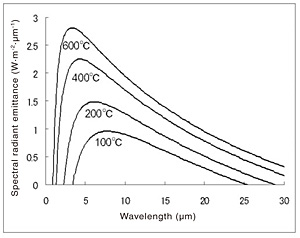
\includegraphics{SpectralEmit.jpg} \\
(ii) Empirical laws -- Wien's Displacement Law:
\begin{equation*}
    \lambda_{max}T = 2.9\times10^{-3}
\end{equation*}
Stefan-Boltzmann Law -- total intensity (Power/Area)
\begin{gather*}
    I = \int_{0}^{\infty} I(\lambda)\,d\lambda = \sigma T^{4} \\
    \sigma = 5.67\times10^{-8}\,\text{W m}^{-2}\,\text{T}^{-4}
\end{gather*}
\textbf{Estimate} the power at which you emit radiation \\
Estimate $A = 1$m$^{2}$
\begin{gather*}
    P = I \times A \\
    ~~ = \sigma \times 1 \times T^{4} \\
    ~~ = \sigma \times (293)^{4} = 410\,W
\end{gather*}

\section{Classical Description}
Radiation caused by oscillating charges, and in equilibrium no net energy is transferred, the net effect means that the radiation in an object (black body cavity) must be a standing wave \\
The number of standing waves in the black body cavity per unit wavelength must be $\propto \frac{1}{\lambda^{3}}$ (one power of $\lambda$ for each dimension) and one more $\lambda$ for 'per unit wavelength', giving:
\begin{equation*}
    I(\lambda) \propto \frac{1}{\lambda^{4}}
\end{equation*}
The full derivation gives:
\begin{equation*}
    I(\lambda) = \frac{2\pi c(kT)}{\lambda^{4}}
\end{equation*}
This seems reasonable at high wavelengths but not at lower ones \\
Gives rise to the \emph{ultra-violet catastrophe}

\section{Planck}
It was noted that the intergral above could be rewritten as a sum \\
It was noted that if the sum wasn't 'infinitesimal' then we could have some mathematical trickery \\
The sum was discritised by assuming that the energy came in discrete packets of $E = hf$ \\
Average energy is total energy divided by number of objects:
\begin{gather*}
    \bar{E} = \frac{\int N(E)E\,dE}{\int N(E)\,dE}
\end{gather*}
N(E) is number of objects with energy E:
\begin{gather*}
    \bar{E} = \frac{\sum_{n = 0}^{\infty} E_{n} N(E_{n})}{\sum_{n=0}^{\infty} N(E_{n})}
\end{gather*}
Boltzmann said that the N(E) is given by:
\begin{gather*}
    N(E) \propto e^{-\tfrac{E}{kT}} \\
    \bar{E} = \frac{0 + hfe^{-\tfrac{hf}{kT}} + 2hfe^{-\tfrac{2hf}{kT}} + \cdots}{1 + e^{-\tfrac{hf}{kT}} + e^{-\tfrac{2hf}{kT}} + \cdots},~~\Big[e^{-\tfrac{hf}{kT}} = x\Big] \implies \\
    \bar{E} = \frac{hfx + 2hfx^{2} + \cdots}{1 + x + x^{2} + \cdots} \\
    ~~ = \frac{hfx}{(1-x)} = \frac{hf}{\tfrac{1}{x} - 1}
    ~~ = \frac{hf}{e^{\tfrac{hf}{kT}} - 1}
\end{gather*}
This resolves for \hl{Planck's Radiation Law}:
\begin{gather*}
    I(\lambda) = \frac{2\pi c}{\lambda^{4}} \frac{hf}{e^{\tfrac{hf}{kT}} - 1} \\
    ~~~~~~ = \frac{2\pi c^{2}}{\lambda^{5}} \frac{h}{e^{\tfrac{hc}{\lambda kT}} - 1}
\end{gather*}
\hl{INTEGRATE AND DIFFERENTIATE THIS} \\
On the discovery of the photoelectric effect, Planck realised his mathematical trick was in fact describing the physics: \\
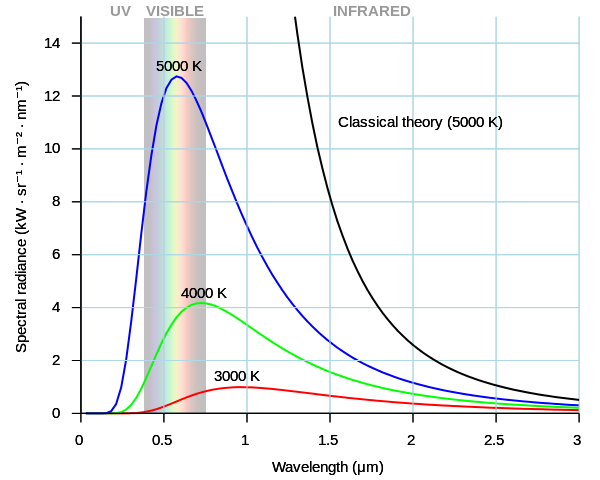
\includegraphics[scale=0.5]{Planck.png}

\section{Wave Equations}
Consider a particle travelling in the x-direction and pretend it's a wave:
\begin{equation*}
    \Psi(x,\,t) = B\cos(kx - \omega t) + C\sin(kx - \omega t)
\end{equation*}
This can also be written as:
\begin{equation*}
    \Psi(x,\,t) = Ae^{i(kx - \omega t)}
\end{equation*}
\begin{itemize}
    \item k -- wave number (rads/meter)
    \item $\omega$ -- frequency (rads/second)
\end{itemize}
\vspace{10pt}
\underline{Particle Properties}
\begin{gather*}
    p = \frac{h}{\lambda} = \hbar k \implies k = \frac{p}{\hbar} \\
    E = hf = \hbar\omega \implies \omega = \frac{E}{\hbar} \\
    \implies \Psi(x,\,t) = Ae^{i\tfrac{px}{\hbar}}e^{-i\tfrac{Et}{\hbar}}
\end{gather*}
What requirements are there for $\Psi$? \\
Conservation of energy:
\begin{gather*}
    E = \frac{p^{2}}{2m} + U \\
    \implies \hbar\omega = \frac{\hbar^{2}k^{2}}{2m} + U
\end{gather*}
\underline{What Else?}
\begin{equation*}
    \Psi = c_{1}\Psi_{1} + c_{2}\Psi_{2}
\end{equation*}
Simplify for now -- call U some constant $V_{0}$
\begin{equation*}
    \Psi(x,\,t) = Ae^{i\tfrac{px}{\hbar}}e^{-i\tfrac{Et}{\hbar}}
\end{equation*}
satisfies wave equation \\
So we have:
\begin{gather*}
    E = \frac{p^{2}}{2m} + V_{0} \\
    E\Psi = \frac{p^{2}}{2m}\Psi + V_{0}\Psi
\end{gather*}
Note the following:
\begin{gather*}
    \frac{\partial \Psi}{\partial t} = Ae^{i\tfrac{px}{\hbar}}\Big(-\frac{iE}{\hbar}\Big)e^{-i\tfrac{Et}{\hbar}} = \Big(-\frac{iE}{\hbar}\Big)\Psi \\
    \frac{\partial \Psi}{\partial x} = A\Big(\frac{ip}{\hbar}\Big)e^{i\tfrac{px}{\hbar}}e^{-i\tfrac{Et}{\hbar}} = \Big(\frac{ip}{\hbar}\Big)\Psi \\
    \frac{\partial^{2} \Psi}{\partial x^{2}} = -\Big(\frac{p}{\hbar}\Big)^{2}\Psi \\
    E\Psi = i\hbar\frac{\partial \Psi}{\partial t} \\
    p^{2}\Psi = -\hbar^{2}\frac{\partial^{2} \Psi}{\partial x^{2}} \\
    i\hbar\frac{\partial \Psi}{\partial t} = -\frac{\hbar^{2}}{2m}\frac{\partial^{2} \Psi}{\partial x^{2}} + V_{0}\Psi
\end{gather*}
Do the same with $V_{0}$ as a function of x and t:

\section{Schr\"{o}dinger's Equation}
\vspace{-20pt}
\begin{equation*}
    i\hbar\frac{\partial \Psi}{\partial t} = -\frac{\hbar^{2}}{2m}\frac{\partial^{2} \Psi}{\partial x^{2}} + U(x,\,t)\Psi(x,\,t)
\end{equation*}

\section{Probability}
Note that the intensity of a wave describes "how big it is" \\
Intensity is given by $|Psi|^{2} = \Psi\cdot\Psi$ which is the probability of finding a particle \\
We have the wave $\Psi(x,\,t)$, then the probability of finding a particle between $x \rightarrow x + dx$ and $t \rightarrow t + dt$ is
\begin{equation*}
    \Psi(x,\,t)\,dx\,dt
\end{equation*}
and if the particle is "somewhere" then:
\begin{equation*}
    \int_{-\infty}^{\infty} \Psi(x,\,t) \cdot \Psi(x,\,t)\,dx = 1
\end{equation*}
Can scale $\Psi$ by a scalar \\
We then get that:
\begin{equation*}
    \int_{-\infty}^{\infty} (A\Psi) \cdot (A\Psi)\,dx = A^{2}
\end{equation*}
Choose A such that $A^{2} = 1$ \\
This is called normalisation \\
If the probabilities sum to one, then we can interpret Schr\"{o}dinger's Equation as giving the probability of finding a particle -- interpretation due to Max Born

\section{A time-independent potential}
Assume that U(x, t) does not vary in time, so is U(x) \\
Note that:
\begin{equation*}
    i\hbar\frac{\partial\Psi}{\partial t} = E\Psi
\end{equation*}
Hence,
\begin{equation*}
    E\Psi = -\frac{\hbar^{2}}{2m}\frac{\partial^{2} \Psi}{\partial x^{2}} + U(x)\Psi(x)
\end{equation*}
Quantum Mechanics (non-relativistic) is governed by Schr\"{o}dinger's Equation \\
For now we will concentrate on understanding the time-independent SE

\section{Infinite Square Well}
\textbf{Example: }Consider a long molecule and it contains an electron which is free to move along the length of the molecule, but does not have enough energy to escape from the molecule \\
Where is the electron and what is its energy? \\
Use SE:
\begin{equation*}
     -\frac{\hbar^{2}}{2m}\frac{d^{2} \Psi(x)}{d x^{2}} + U(x)\Psi(x) = E\Psi(x)
\end{equation*}
Electron is free to move inside the molecule so but cannot leave the molecule so:
\begin{gather*}
    U(x) =
    \begin{cases}
        0,      & 0 \leq x \leq L \\
        \infty, & x < 0,~x > L
    \end{cases}
\end{gather*}
Outside bounds, $P = 0$, $\Psi(x) = 0$ \\
Inside bounds, potential is 0, hence SE is:
\begin{gather*}
    -\frac{\hbar^{2}}{2m}\frac{d^{2} \Psi(x)}{d x^{2}} + U(x)\Psi(x) = E\Psi(x) \\
    \frac{d^{2} \Psi(x)}{d x^{2}} = -\frac{2mE}{\hbar^{2}}\Psi(x) \\
    \Big[\frac{2mE}{\hbar^{2}} = k^{2}\Big] \implies \\
    \frac{d^{2} \Psi(x)}{d x^{2}} = -k^{2}\Psi(x)
\end{gather*}
A solution to this is
\begin{equation*}
    \Psi(x) = B\cos(kx) + C\sin(kx)
\end{equation*}
Can use boundary conditions to find constants:
\begin{gather*}
    \Psi(0) = 0 \implies \Psi(0) = B\cos(0) + C\sin(0) = 0 \\
    \therefore ~ B = 0 \\
    \Psi(L) = 0 \implies \Psi(L) = C\sin{kL} = 0 \\
    \therefore ~ kL = n\pi,~n \in \mathbb{Z} \\
    \therefore ~ k_{n} = \frac{n\pi}{L} \\
    k_{n}^{2} = \frac{2mE_{n}}{\hbar^{2}} \\
    \therefore ~ E_{n} = \frac{n^{2}\pi^{2}\hbar^{2}}{2mL^{2}}
\end{gather*}
Energies are quantised \\
Solve for wave function:
\begin{equation*}
    \Psi_{n}(x) = C\sin\Big(\frac{n\pi x}{L}\Big),~0 \leq x \leq L
\end{equation*}
Normalise the wave function: For $|\Psi|^{2}$ to describe the probability, we require the total probability to sum to 1
\begin{gather*}
    \int_{-\infty}^{\infty} |\Psi|^{2}\,dx = 1 \\
    1 = \int_{-\infty}^{\infty} \rightarrow \Bigg(\int_{-\infty}^{0} = 0\Bigg) + \int_{0}^{L} + \Bigg(\int_{L}^{\infty} = 0\Bigg) \\
    1 = \int_{0}^{L} C^{2}\sin^{2}\Big(\frac{n\pi x}{L}\Big)\,dx \\
    \Big[\sin^{2} = \frac{1}{2}(1 - \cos(2x))\Big] \\
    1 = \frac{C^{2}L}{2} \implies C = \sqrt{\frac{2}{L}} \\
    \Psi_{n}(x) = \sqrt{\frac{2}{L}}\sin\Big(\frac{n\pi x}{L}\Big)
\end{gather*}
Plots of $\Psi$ on left, $|\Psi|^{2}$ on right: \\
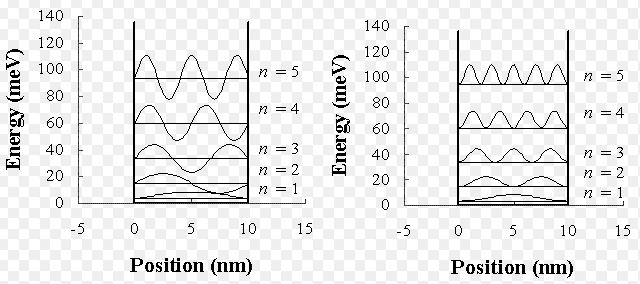
\includegraphics{Squarez.jpg} \\
To get from Quantum to Classical, make n big

\section{Notes on Infinite Square Well}
(i) Ground state can be estimated from Heisenberg:
\begin{gather*}
    \Delta x = L \rightarrow \Delta p \approx \frac{\hbar}{2L} \\
    \text{Energy is KE so }\Delta E = \frac{(\Delta p)^{2}}{2m} \approx \frac{\hbar^{2}}{8mL^{2}}
\end{gather*}
(ii) The wavefunctions are perpendicular:
\begin{gather*}
    \int_{-\infty}^{\infty} \Psi_{n}^{\ast}(x)\cdot\Psi_{m}(x) = \delta_{nm}
    \begin{cases}
        0, & n \neq m \\
        1, & n = m
    \end{cases} \\
    \frac{2}{L}\int_{0}^{L}\sin\Big(\frac{n\pi x}{L}\Big)\sin\Big(\frac{m\pi x}{L}\Big)\,dx = \delta_{nm}
\end{gather*}
-- Pauli Exclusion Principle \\
(Swapping)
\begin{gather*}
    S\cdot\Psi(r_{1},\,r_{2}) = X\cdot\Psi(r_{2},\,r_{1}) \\
    S^{2}\cdot\Psi(r_{1},\,r_{2}) = \Psi(r_{2},\,r_{1}) \\
    S^{2} = 1,~S = \pm 1 \\
    \Psi(r_{1},\,r_{2}) = \Psi(r_{2},\,r_{1}) \rightarrow \text{Bosons} \\
    \Psi(r_{1},\,r_{2}) = -\Psi(r_{2},\,r_{1}) \rightarrow \text{Fermions}
\end{gather*}
(iii) $\Psi_{n}(x) = \sqrt{\frac{2}{L}}\sin\Big(\frac{n\pi x}{L}\Big)$ -- Fourier series? \\
If $\Psi_{n}(x)$ and $\Psi_{m}(x)$ are solutions to SE, so is $a\Psi_{n}(x) + b\Psi_{m}(x)$ \\
But then so must be:
\begin{gather*}
    \Psi(x) = \sum_{n = 1}^{\infty} c_{n}\cdot\Psi_{n}{x} \\
    \Psi(x) = \sum_{n = 1}^{\infty} c_{n}\cdot\sin\Big(\frac{n\pi x}{L}\Big)
\end{gather*}
-- is general solution

(iv) Solving for time-dependent:
\begin{equation*}
    \Psi(x,\,t) = \Psi_{n}(x)e^{-i\tfrac{E_{n}t}{\hbar}}
\end{equation*}
There is no difference to the probability function

\section{Example in Infinite Square Well}
Energy values?
\begin{gather*}
    \Psi(x) = \sin\Big(\frac{\pi x}{L}\Big)\cos\Big(\frac{2\pi x}{L}\Big) \\
    \Psi(x) = \frac{1}{2}\sin\Big(\frac{3\pi x}{L}\Big) - \frac{1}{2}\sin\Big(\frac{\pi x}{L}\Big) \\
    \Psi(x) = \frac{1}{2}\Psi_{3}(x) - \frac{1}{2}\Psi_{1}(x) \\
    \text{Energies: }
    \begin{cases}
        n = 1 \rightarrow& E_{1} = \dfrac{\pi^{2}\hbar{2}}{2mL^{2}} \\
        n = 3 \rightarrow& E_{3} = \dfrac{9\pi^{2}\hbar^{2}}{2mL^{2}}
    \end{cases}
\end{gather*}
Notes: Coefficients are equal so equal probability \\
This is not very physical -- make potential well finite:

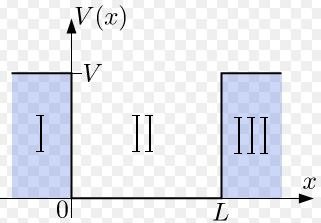
\includegraphics{Finite.jpg} \\
More realistic potential \\
Try to solve SE of this system, need to deal with constants of integration and so we need boundary conditions \\
To desribe a real potential, normalise:
\begin{gather*}
    \int_{-\infty}^{\infty} |\Psi|^{2}\,dx = 1 \\
    \Psi(x) \rightarrow 0 \text{ as } x \rightarrow \pm\infty
\end{gather*}
E is finite so $\frac{d^{2}\Psi}{dx^{2}}$ must be finite \\
Therefore, $\Psi(x)$ and $\frac{d\Psi}{dx}$ are continuous \\
Inside box:
\begin{gather*}
    \Psi_{II}(x) = A\cos(kx) + B\sin(kx)
\end{gather*}
Outside box:
\begin{gather*}
    \frac{d^{2}\Psi_{I}(x)}{dx^{2}} = \frac{2m}{\hbar^{2}}(V - E)\Psi = \kappa^{2}\Psi \\
    \kappa^{2} = \frac{2m}{\hbar^{2}}(V -E) \\
    \Psi_{I}(x) = \alpha e^{\kappa x} + \beta e^{-\kappa x} \\
    \Psi_{III}(x) = \gamma e^{\kappa x} + \delta e^{-\kappa x}
\end{gather*}
$\beta$ and $\gamma = 0$ due to infinities \\
Did not calculate energies explicitly but can bound them:
\begin{figure}[H]
    \begin{subfigure}{0.18\textwidth}
        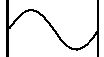
\includegraphics{n=2.jpg}
        \caption{$\infty,~n = 2$}
    \end{subfigure}
    \begin{subfigure}{0.30\textwidth}
        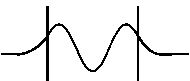
\includegraphics{n=3.jpg}
        \caption{$n = 3$}
    \end{subfigure}
    \begin{subfigure}{0.2\textwidth}
        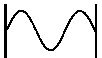
\includegraphics{infty3.jpg}
        \caption{$\infty,~n = 3$}
    \end{subfigure}
\end{figure}
\begin{gather*}
    E_{2}^{\infty} = \frac{2^{2}\pi^{2}\hbar^{2}}{2mL^{2}} < E_{3}^{f} < E_{3}^{\infty} = \frac{3^{2}\pi^{2}\hbar^{2}}{2mL^{2}}
\end{gather*}
Or in terms of wave number:
\begin{equation*}
    \frac{2\pi}{L} < k_{3}^{f} < \frac{3\pi}{L}
\end{equation*}
Energy of particle $E < V$ where E is $E_{n}^{f}$ but there must be an n for which $E_{n}^{f} > V$ -- there are a finite number of bound states \\
As we increase n, eventually $E_{n}^{f} > V$ and we have the case of a free particle

\section{Potential Barriers}
Consider a particle travelling to the right approaching a potential barrier:
\begin{gather*}
    U(x) =
    \begin{cases}
        0,     & x < 0 \\
        U_{0}, & x \geq 0
    \end{cases}
\end{gather*}
$\underline{E < U_{0}}$ \\
$\mathbf{x < 0}~(U(x) = 0)$
\begin{gather*}
    \frac{d^{2}\Psi_{L}}{dx^{2}} = -\frac{2mE}{\hbar^{2}}\Psi_{L} \\
    ~~~~~~~~ = -k^{2}\Psi_{L} \\
    \Psi_{L}(x) = \overrightarrow{A}e^{ikx} + \overleftarrow{B}e^{-ikx}
\end{gather*}
\begin{itemize}
    \item A -- left to right, incident wave
    \item B -- right to left, reflected wave
\end{itemize}
$\mathbf{x \geq 0}~(U(x) = U_{0})$
\begin{gather*}
    \frac{d^{2}\Psi_{R}}{dx^{2}} = -\frac{2m(E - U_{0})}{\hbar^{2}}\Psi_{R} \\
    ~~~~~~~~ = \kappa^{2}\Psi_{R} \\
    \Psi_{R}(x) = Ce^{-\kappa x} + De^{\kappa x}
\end{gather*}
\begin{itemize}
    \item C -- exponential decay into barrier
    \item D -- exponential increase into barrier, must be 0
\end{itemize}
Continuity at $x = 0$ means that:
\begin{gather*}
    \Psi_{L}(0) = \Psi_{R}(0) \\
    A + B = c
\end{gather*}
Continuity in the derivatives:
\begin{gather*}
    \frac{d\Psi_{L}}{dx}\Big|_{x = 0} = \frac{d\Psi_{R}}{dx}\Big|_{x = 0} \\
    \implies ik(A - B) = -\kappa C \\
    \frac{C}{A} = \frac{2k}{k + i\kappa},~~~\frac{B}{A} = \frac{k - i\kappa}{k + i\kappa}
\end{gather*}
$|\frac{B}{A}|^{2}$ -- ratio of incoming particles to reflected, called the reflection coefficient \\
$|\frac{C}{A}|^{2}$ -- ratio of incoming particles to transmitted, call the transmission coefficient

$\underline{E > U_{0}}$ \\
$\mathbf{x < 0}~(U(x) = 0)$
\begin{equation*}
    \Psi_{L}(x) = \overrightarrow{A}e^{ikx} + \overleftarrow{B}e^{-ikx}
\end{equation*}
$\mathbf{x > 0}~(U(x) = U_{0})$
\begin{gather*}
    \Psi_{R}(x) = \big(\overleftarrow{C}e^{-i\kappa x} = 0\big) + \overrightarrow{D}e^{i\kappa x} \\
    ~~~~~~~~ = \Psi_{R}(x) = De^{i\kappa x} \\
\end{gather*}
Coefficients:
\begin{gather*}
    \frac{D}{A} = \frac{2k}{k + \kappa} \\
    \frac{B}{A} = \frac{k - \kappa}{k + \kappa}
\end{gather*}
\textbf{Example:} \\
Potential barrier between 0 and L \\
Particle came from left with $E < U_{0}$:
\begin{gather*}
    \RN{1} \implies \Psi_{\RN{1}}(x) = Ae^{ikx} + Be^{-ikx} \\
    \RN{2} \implies \Psi_{\RN{2}}(x) = Ce^{\kappa x} + De^{-\kappa x} \\
    \RN{3} \implies \Psi_{\RN{3}}(x) = Fe^{ikx} + \cancel{Ge^{-ikx}}
\end{gather*}
A is determined through normalisation \\
Other constants through boundaries
\begin{gather*}
    \Psi_{\RN{1}}(0) = \Psi_{\RN{2}}(0)~~~~\&~~~\Psi_{\RN{2}}(L) = \Psi_{\RN{3}}(L) \\
    \frac{d\Psi_{\RN{1}}}{dx}\Big|_{0} = \frac{d\Psi_{\RN{2}}}{dx}\Big|_{0}~~\&~~\frac{d\Psi_{\RN{2}}}{dx}\Big|_{L} = \frac{d\Psi_{\RN{3}}}{dx}\Big|_{L}
\end{gather*}
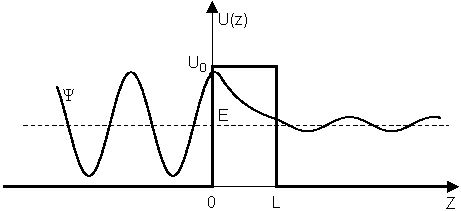
\includegraphics{PotBar.jpg} \\
We have the usual coefficients at $x = 0$ as well as an extra one for the transmission coefficient through the full barrier: $|\frac{F}{A}|^{2}$ \\
This is a reasonable model for a transistor

\textbf{Example: }sinusoidal motion has $\omega = \sqrt{\frac{k}{m}}$, amplitude A \\
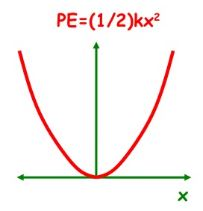
\includegraphics{Pote.jpg} \\
If particle has energy E, at extremes, E is desrcibed by PE
\begin{gather*}
    x = A \implies PE = \frac{1}{2}kA^{2} \\
    x = 0 \implies KE = \frac{1}{2}mv^{2} = \frac{1}{2}kA^{2}
\end{gather*}
\underline{Question}
\begin{equation*}
    -\frac{\hbar^{2}}{2m}\frac{d^{2}\Psi(x)}{dx^{2}} + \frac{1}{2}kx^{2}\Psi(x) = E\Psi(x)
\end{equation*}
This is "a pain in the arse" to solve \\
So jump straight to solutions for now: \\
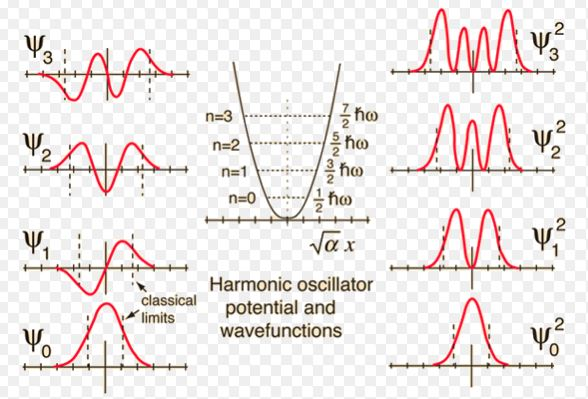
\includegraphics{HarmOsc.jpg} \\
Solve SE for SHO:
\begin{gather*}
    \Psi_{1}(x) = e^{-\tfrac{m\omega x^{2}}{2\hbar}}\text{ (Gaussian)} \\
    \Psi_{2}(x) \approx xe^{-x^{2}}\text{ ... plus some constants}
\end{gather*}
In general:
\begin{gather*}
    \Psi_{n}(x) = A_{n}(1 + c_{1}x + c_{2}x^{2} + \cdots + c_{n}x^{n})e^{-\tfrac{m\omega x^{2}}{2\hbar}} \\
    E_{n} = \bigg(n + \frac{1}{2}\bigg)\hbar\omega
\end{gather*}
For $\Psi_{big}(x)$, similar image to $\frac{\sin(x)}{x}$ -- tends to classical solution \\
When $n = 0$, $E_{0} = \frac{1}{2}\hbar\omega$ \\
There is a solution for $E = 0$ \\
Heisenberg comes from this:
\begin{gather*}
    E = \frac{1}{2}\hbar\omega = \frac{1}{2}\hbar\frac{1}{T} \\
    T\cdot E = \frac{\hbar}{2}
\end{gather*}

\section{3D Schr\"{o}dinger}
Momemtum is a vector so we can rewrite KE:
\begin{gather*}
    KE = \frac{p_{x}^{2}}{2m} + \frac{p_{y}^{2}}{2m} + \frac{p_{z}^{2}}{2m} \\
    \Psi(x,\,y,\,z) = e^{\tfrac{i}{\hbar}\underline{p}\cdot\underline{x}} = e^{\tfrac{i}{\hbar}(p_{x}x + p_{y}y + p_{z}z)}
\end{gather*}
Can take various derivatives, $p_{x} \rightarrow -i\hbar\frac{\partial}{\partial x}$ \\
SE:
\begin{gather*}
    -\frac{\hbar^{2}}{2m}\Bigg[\frac{\partial^{2}\Psi(x,\,y,\,z)}{\partial x} + \frac{\partial^{2}\Psi(x,\,y,\,z)}{\partial y} + \frac{\partial^{2}\Psi(x,\,y,\,z)}{\partial z}\Bigg] + U(x,\,y,\,z)\Psi(x,\,y,\,z) = E\Psi(x,\,y,\,z) \\
    \frac{\hbar^{2}}{2m}\nabla^{2}\Psi + U\Psi = E\Psi
\end{gather*}

\section{Particle In A Box In 3D}
\vspace{-22pt}
\begin{gather*}
    U(x,\,y,\,z) =
    \begin{cases}
        0, & 0 \leq x,\,y,\,z \leq L \\
        \infty, & \text{Otherwise}
    \end{cases} \\
    \Psi(x/y/z = 0) = \Psi(x/y/z = L) = 0
\end{gather*}
This is a simple enough situation that equation is separable:
\begin{equation*}
    \Psi(x,\,y,\,z) = X(x)Y(y)Z(z)
\end{equation*}
Now some maths:
\begin{gather*}
    X''YZ + Y''XZ + Z''XY = -k^{2}XYZ,~~k^{2} = \frac{2mE}{\hbar^{2}} \\
    \Big[\times \frac{1}{XYZ}\Big] \\
    \frac{1}{X}X'' + \frac{1}{Y}Y'' + \frac{1}{Z}Z'' = -k^{2}
\end{gather*}
Independent solutions so:
\begin{gather*}
    X'' = -k_{x}^{2}X,~~~Y'' = -k_{y}^{2}Y,~~~Z'' = -k_{z}^{2}Z \\
    X = A\sin\bigg(\frac{n_{x}\pi x}{L_{x}}\bigg),~~Y = B\sin\bigg(\frac{n_{y}\pi y}{L_{y}}\bigg),~~Z = C\sin\bigg(\frac{n_{z}\pi z}{L_{z}}\bigg) \\
    \bigg[k_{i} = \frac{n_{i}\pi}{L} \implies \bigg] \\
    \Psi(x,\,y,\,z) = D\sin\bigg(\frac{n_{x}\pi x}{L_{x}}\bigg)\sin\bigg(\frac{n_{y}\pi y}{L_{y}}\bigg)\sin\bigg(\frac{n_{z}\pi z}{L_{z}}\bigg) \\
    E = \frac{\hbar^{2}\pi^{2}}{2m}\Big(\frac{n_{x}^{2} + n_{y}^{2} + n_{z}^{2}}{L}\Big)\text{ -- Cube} \\
    E = \frac{\hbar^{2}\pi^{2}}{2m}\Big(\frac{n_{x}^{2}}{L_{x}^{2}} + \frac{n_{y}^{2}}{L_{y}^{2}} + \frac{n_{z}^{2}}{L_{z}^{2}}\Big)\text{ -- Cuboid}
\end{gather*}
Number of dimensions is the number of quantum numbers:
\begin{equation*}
    E_{1,1,2} = E_{1,2,1} = E_{2,1,1}
\end{equation*}
These equivalent energies are called degenerate orbitals

\textbf{Example: }3D particle in box, maximum for (1, 1, 1) and (2, 2, 1) \\
Max for:
\begin{gather*}
    |\Psi(x,\,y,\,z)|^{2} \\
    \Psi \propto \sin\bigg(\frac{n_{x}\pi x}{L_{x}}\bigg)\sin\bigg(\frac{n_{y}\pi y}{L_{y}}\bigg)\sin\bigg(\frac{n_{z}\pi z}{L_{z}}\bigg)
\end{gather*}
For (1, 1, 1):
\begin{gather*}
    \sin\bigg(\frac{\pi x}{L_{x}}\bigg)\sin\bigg(\frac{\pi y}{L_{y}}\bigg)\sin\bigg(\frac{\pi z}{L_{z}}\bigg) \\
    \frac{\pi x}{L} = \frac{\pi y}{L} = \frac{\pi z}{L} = \frac{\pi}{2} \\
    (x,\,y,\,z) = \bigg(\frac{L}{2},\,\frac{L}{2},\,\frac{L}{2}\bigg)
\end{gather*}
For (2, 2, 1):
\begin{gather*}
    \sin\bigg(\frac{2\pi x}{L_{x}}\bigg)\sin\bigg(2\frac{\pi y}{L_{y}}\bigg)\sin\bigg(\frac{\pi z}{L_{z}}\bigg) \\
    \frac{2\pi x}{L} = \frac{2\pi y}{L} = \frac{\pi}{2} = \frac{\pi z}{L} \\
    (x,\,y,\,z) = L\bigg(\frac{1}{4},\frac{1}{4},\frac{1}{2}\bigg),~~ L\bigg(\frac{1}{4},\frac{3}{4},\frac{1}{2}\bigg),~~ L\bigg(\frac{3}{4},\frac{1}{4},\frac{1}{2}\bigg),~~
    L\bigg(\frac{3}{4},\frac{3}{4},\frac{1}{2}\bigg)
\end{gather*}
\textbf{Example: }Pretend hydrogen atom is a cube with same volume as a "Bohr sphere" \\
What is the energy lost from the first excited state to ground state?
\begin{gather*}
    L^{3} = \frac{4}{3}\pi a^{3},~~a \approx 0.52\text{\r{A}} \\
    L \approx 8.53\times10^{-11}m \\
    E_{2,1,1} - E_{1,1,1}: \\
    \frac{\hbar^{2}\pi^{2}}{2mL^{2}}[(2^{2} + 1^{2} + 1^{2}) - (1^{2} + 1^{2} + 1^{2})] = 1.55\,eV
\end{gather*}
The real answer for hydrogen is about 10.2\,eV \\
Cube is not a good approximation

\section{The Hydrogen Atom}
Can be considered to be a sphere of radius $r = \sqrt{x^2 + y^2 + z^2}$ with an electron potential given from Coulomb's Law:
\begin{equation*}
    V(x,\,y,\,z) = \frac{-e^{2}}{4\pi\epsilon_{0}\sqrt{x^2 + y^2 + z^2}}
\end{equation*}
Write SE and then use spherical polars to simplify problem:
\begin{gather*}
    -\frac{\hbar^{2}}{2m}\nabla^{2}\Psi(x,\,y,\,z) + \frac{-e^{2}}{4\pi\epsilon_{0}\sqrt{x^2 + y^2 + z^2}}\Psi(x,\,y,\,z) = E\Psi(x,\,y,\,z) \\
    \bigg[\cos\theta = \frac{x}{r},~\tan\phi = \frac{y}{x}\bigg] \implies \\
    \nabla^{2} = \frac{1}{r^{2}}\frac{\partial}{\partial r}\Big(r^{2}\frac{\partial}{\partial r}\Big) + \frac{1}{r^{2}\sin\theta}\frac{\partial}{\partial\theta} \Big(\sin\theta \frac{\partial}{\partial\theta}\Big) + \frac{1}{r^{2}\sin\theta}\frac{\partial^{2}}{\partial \Psi^{2}} \\
    \Psi(x,\,y,\,z) \rightarrow R(r)\Theta(\theta)\Phi(\phi)
\end{gather*}
This results in three quantum numbers:
\begin{itemize}
    \item n -- principle quantum number
    \item l -- angular momentum quantum number
    \item $m_{l}$ -- magnetic quantum number
\end{itemize}
The three equations are:
\begin{gather*}
    -\frac{\hbar^{2}}{2m}\frac{1}{r^{2}}\frac{d}{dr}\bigg(r^{2}\frac{dR_{n}(r)}{dr}\bigg) + \bigg(\frac{\hbar^{2}l(l + 1)}{2m} + U(r)\bigg)R_{n}(r) = E_{n}R_{n}(r) \\
    \frac{1}{\sin\theta}\frac{d}{d\theta}\bigg(\sin\theta \frac{d\Theta(\theta)}{d\theta}\bigg) + \bigg(l(l + 1) - \frac{m_{l}^{2}}{\sin^{2}\theta}\bigg)\Theta(\theta) = 0 \\
    \frac{d^{2}\Phi(\phi)}{d\phi^{2}} + m_{l}^{2}\Phi(\phi) = 0
\end{gather*}
Solving these equations gives the following rules:
\begin{gather*}
    n = 1,\,2,\,3,\,4,\, \cdots \\
    l = 0,\,1,\,2,\, \cdots ,\,(n - 1) \\
    -l \leq m_{l} \leq l
\end{gather*}
Solve 3 differentials:
\begin{equation*}
    \Psi(x,\,y,\,z) = R(r)\Theta(\theta)\Phi(\phi)
\end{equation*}
Notation for n then l:
\begin{table}[H]
    \begin{tabular}{c|ccccc}
        Physics   & 1 & 2 & 3 & 4 & ...   \\
        Chemistry & K & L & M & N & ...   \\
        \hline
        \hline
        Physics   & 0 & 1 & 2 & 3 & 4... \\
        Chemistry & s & p & d & f & g...
    \end{tabular}
\end{table}
s -- sharp; p -- principle; d -- diffuse; f -- fine \\
From Schr\"{o}dinger Equation:
\begin{equation*}
    |\underline{L}| = \sqrt{l(l + 1)}\hbar
\end{equation*}
For electrons in shells with $l = 0$, $|\underline{L}| = 0$

\section{Magnetic Quantum Number}
Bohr had $E \propto \frac{1}{n^{2}}$ -- Energy is at discrete levels \\
In SE solution, there are multiple degenerate levels (with the same energy) \\
Consider spectral lines:
\begin{figure}[H]
    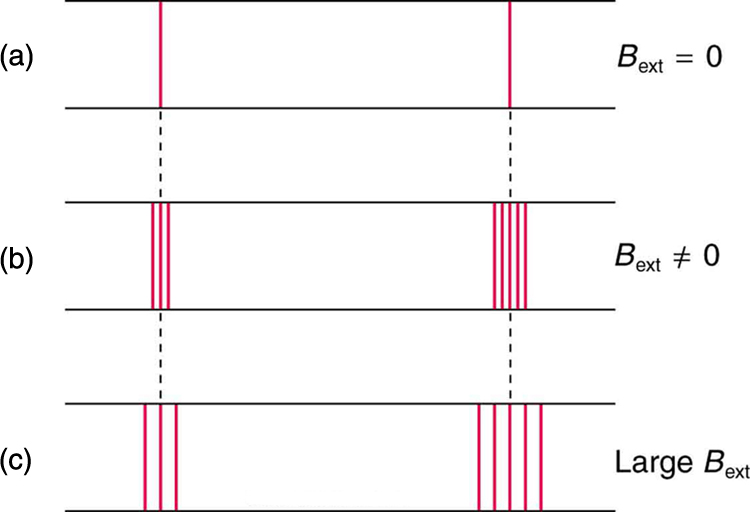
\includegraphics{MLS.jpg}
\end{figure}
\begin{gather*}
    \underline{\mu} = IA \\
    U = -\underline{\mu}\cdot\underline{B} \\
    T = \frac{2\pi r}{v} \implies I = \frac{e}{T} = \frac{qv}{2\pi r} \\
    |L| = mvr \implies \\
    |\mu| = IA = \frac{qv}{2\cancel{\pi}\cancel{r}}\cancel{\pi}r^{\cancel{2}} = \frac{1}{2}qvr = \frac{qvrm}{2m} = \frac{e}{2m}|\underline{L}| \\
    \mu = -\frac{e}{2m}|\underline{L}| \\
    U = -\mu \cdot B = \frac{e}{2m}\underline{L} \cdot \underline{B} = \frac{e}{2m}L_{z}B_{z} = \frac{e}{2m}m_{l}m_{l}\hbar B_{z} \\
    \bigg[\mu_{B} = \frac{e\hbar}{2m}\bigg] \\
    U = \mu_{B}m_{l}B_{z}
\end{gather*}
This was the Zeeman effect for splitting of the spectrum \\
Until observation of splitting at $l = 0$ \\
Have to quantise $L_{z}$ differently for it to work \\
There is an intrinsic angular momentum associated with fundamental particles, known as spin \\
Let \underline{S} be intrinsic angular momentum, then $\underline{\mu} = \frac{e}{2m}\underline{S}$ \\
Quantise $\underline{S}$: two values $\rightarrow m_{s} = \pm \frac{1}{2}$ \\
This explains two lines \\
These two spin states are usually referred to as up for positive or down for negative
\begin{equation*}
    \mu_{z} = -m_{s}\mu_{B}
\end{equation*}
There is a factor of two to deal with, called the electron gyromagnetic ratio \\
Measured as slightly more than two to about 14 decimal places -- forgot relativity
\begin{equation*}
    \underline{J} = \underline{L} + \underline{S}
\end{equation*}
What values of $m_{s}$ for $l = 1$?
\begin{gather*}
    m_{l} = -1,\,0,\,1 ~~~ m_{s} = \pm \frac{1}{2} \\
    m_{j} = -\frac{3}{2},\,-\frac{1}{2},\,\frac{1}{2},\,-\frac{1}{2},\,\frac{1}{2},\,\frac{3}{2}
\end{gather*}

\section{For Many Electrons...}
Write down SE for Helium atom \\
Nucleus of charge +2e and 2 electrons in orbit \\
Origin at nucleus:
\begin{equation*}
    \Bigg[-\frac{\hbar^{2}}{2m}\Big(\frac{\partial^{2}}{\partial x_{1}^{2}} + \frac{\partial^{2}}{\partial y_{1}^{2}} + \frac{\partial^{2}}{\partial z_{1}^{2}}\Big) - \frac{2e^{2}}{4\pi\epsilon_{0}|r_{1}|} - \frac{\hbar^{2}}{2m}\Big(\frac{\partial^{2}}{\partial x_{2}^{2}} + \frac{\partial^{2}}{\partial y_{2}^{2}} + \frac{\partial^{2}}{\partial z_{2}^{2}}\Big) - \frac{2e^{2}}{4\pi\epsilon_{0}|r_{2}|} + \frac{e^{2}}{4\pi\epsilon_{0}|r_{12}|}\Bigg] \times \Psi(r_{1},\,r_{2}) = E\Psi(r_{1},\,r_{2})
\end{equation*}
The final term inside the square brackets makes it impossible to solve under normal techniques, otherwise it is separable \\
Pauli Exclusion Principle gives negative sign if swapping electrons in SE \\
Ignoring that final term for solving, gives solution without this negative

\section{Pauli Exclusion Principle}
\emph{"No two electrons can occupy the same quantum state"} -- only one electron in a system can have a given set of quantum numbers
\begin{table}[H]
    \begin{tabular}{c|ccc|c}
        n & l & $m_{l}$ & $m_{s}$ & Label \\
        \hline
        1 & 0 & 0 & $\pm \frac{1}{2}$ & $1s^{2}$ \\
        2 & 0 & 0 & $\pm \frac{1}{2}$ & $2s^{2}$ \\
        2 & 1 & -1,\,0,\,1 & $\pm \frac{1}{2}$ & $2p^{6}$ \\
        3 & 0 & 0 & $\pm \frac{1}{2}$ & $3s^{2}$ \\
        3 & 1 & -1,\,0,\,1 & $\pm \frac{1}{2}$ & $3p^{6}$ \\
        3 & 2 & -2,\,-1,\,0,\,1,\,2 & $\pm \frac{1}{2}$ & $3d^{10}$
    \end{tabular}
\end{table}

\section{SE of Everything}
In the Universe, let's have N nuclei, m electrons (upper case for nuclei and lower case for electrons):
\begin{multline*}
    \Bigg[\underset{\text{KE Nuclei}}{\sum_{I = 1}^{N}-\frac{\hbar^{2}}{2M_{I}}\nabla^{2}} + \underset{\text{KE electrons}}{\sum_{j = 1}^{m}-\frac{\hbar^{2}}{2m} \nabla^{2}} \underset{\text{Coulomb} \rightarrow}{- \frac{1}{4\pi\epsilon_{0}}} \underset{elec--nuc}{\sum_{I = 1}^{N}\sum_{j = 1}^{m}\frac{Z_{I}e^{2}}{|R_{I} - r_{j}|}} + \underset{elec--elec}{\frac{1}{2}\sum_{i = 1}^{m}\sum_{j = 1}^{m}\frac{e^{2}}{4\pi\epsilon_{0}|r_{i} - r_{j}|}} + \underset{nuc--nuc}{\frac{1}{2}\sum_{I = 1}^{N}\sum_{J = 1}^{N}\frac{Z_{J}Z_{I}e^{2}}{4\pi\epsilon_{0}|R_{I} - R_{J}|}}\Bigg] \\
    \times \Psi(R_{1},\,R_{2},\, \cdots ,\,R_{N},\,r_{1},\,r_{2},\, \cdots ,\,r_{m}) = E\Psi(R_{1},\,R_{2},\, \cdots ,\,R_{N},\,r_{1},\,r_{2},\, \cdots ,\,r_{m})
\end{multline*}

\newpage
\section{Atomic Nucleus}
Basic properties:
\begin{table}[H]
    \begin{tabular}{c|c|c}
               & Proton & Neutron   \\
        \hline
        Charge & +1     & 0         \\
        Mass ($\frac{MeV}{c^{2}}$)  & 938.3  & 939.6   \\
        Spin   & $\frac{1}{2}$ & $\frac{1}{2}$ \\
        Lifetime & Stable & 918s
    \end{tabular}
\end{table}
Symbol Z for atomic number $\implies A = Z + N$, A is the mass number \\
A nuclear species is a nuclide \\
An isotope contains a given number of protons but neutrons vary \\
An isotone has the same number of neutrons but protons vary \\
An isobar has the same mass number but neutrons and protons vary \\
We have a number of positive protons in the nucleus that repel via the Coulomb force \\
Why doesn't the nucleus blow apart? \\
THere is another force:
\begin{enumerate}
    \item It must be stronger than the Coulomb force
    \item It must be short range
    \item It must "saturate" at some point, at short range
\end{enumerate}

\section{Nuclear Stability}
Some nuclei and we observe:
\begin{enumerate}
    \item $\alpha$ particles -- $_{2}^{4}$He
    \item $\beta$ particles -- e$^{-}$
    \item $\gamma$ decay -- photons
    \item proton or neutron decay
\end{enumerate}

\section{Half-Life}
Let N(t) be the number of nucleons of a species that exist in a sample time, t \\
Let $\lambda$ be the rate at which they are observed to decay \\
It appears that the rate of change of N(t) is $\propto \lambda$:
\begin{equation*}
    \frac{dN(t)}{dt} = -\lambda N(t)
\end{equation*}
So if we let $N(0) = N_{0}$, then solving this differential gives us:
\begin{equation*}
    N(t) = N_{0}e^{-\lambda t}
\end{equation*}
The half-life is the time taken for $N_{0}$ to decay to $\frac{N_{0}}{2}$:
\begin{equation*}
    \frac{N(t)}{N_{0}} = \frac{1}{2} = e^{-\lambda t_{1/2}} \implies t_{1/2} = \frac{\ln{2}}{\lambda}
\end{equation*}

\newpage
\section{What determines $\lambda$?}
If we examine the properties that are required for the nuclear force then we can construct a model nuclear potential:
\begin{figure}[H]
    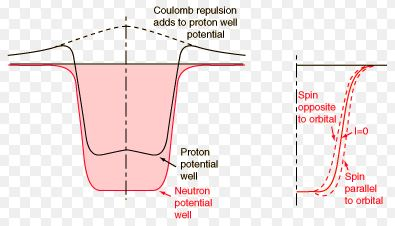
\includegraphics{lamb.jpg}
\end{figure}
In a stable nucleus, the energy levels are bound

$_{2}^{4}$He is very tightly bound and takes up energy to break up so there is less energy involved in emitting the full thing so more common than single neutron/proton decay

$\gamma$ decay -- nucleus has energy levels, just like atom \\
If we excite the nucleus into a higher state, at some point, it will decay back into the ground state by releasing a photon [perturbation theory]

$\beta$ decay -- similar to neutron potential well

\section{Relativistic Quantum Mechanics}
Relativity:
\begin{equation*}
    E^{2} = p^{2}c^{2} + m_{0}^{2}c^{4} ~~ (1) \\
\end{equation*}
Quantum:
\begin{equation*}
    E = \frac{p^{2}}{2m} \rightarrow SE
\end{equation*}
Go from (1) to SE:
\begin{gather*}
    E^{2} + c^{2}(-p_{x}^{2} - p_{y}^{2} - p_{z}^{2}) - c^{4}m_{0}^{2} = 0 \\
    \implies \cdots \\
    \frac{1}{c^{2}}\frac{\partial^{2}\Psi}{\partial t^{2}} - \nabla^{2}\Psi + \frac{m_{0}^{2}c^{2}}{\hbar^{2}}\Psi = 0
\end{gather*}
This is called the Klein-Gordon equation, and it doesn't work \\
Using this in highly relativistic settings, probability density can be negative \\
This comes from $\frac{\partial^{2}\Psi}{\partial t^{2}}$ which in turn comes from:
\begin{equation*}
    E = \pm\sqrt{p^{2}c^{2} + m_{0}^{2}c^{4}}
\end{equation*}
Need first order term instead to fix this:
\begin{gather*}
    E^{2} = p^{2}c^{2} + m_{0}^{2}c^{4} \\
    ~~~ = (\gamma_{0}E + \gamma_{1}p_{x} + \gamma_{2}p_{y} + \gamma_{3}p_{z} - m) \times (\gamma_{0}E + \gamma_{1}p_{x} + \gamma_{2}p_{y} + \gamma_{3}p_{z} + m) \\
    \implies \\
    \gamma_{0}^{2} = 1 \\
    \gamma_{1}^{2} = \gamma_{2}^{2} = \gamma_{3}^{2} = -1 \\
    \gamma_{i}\gamma_{j} = -\gamma_{j}\gamma_{i}
\end{gather*}
Can use matrices to make sure these come out \\
We get $4 \times 4$ matrices:
\begin{equation*}
    \Bigg[\gamma_{0}\frac{\partial}{\partial t} - \gamma_{1}\frac{\partial}{\partial x} - \gamma_{2}\frac{\partial}{\partial y} - \gamma_{3}\frac{\partial}{\partial z} - \frac{1}{i\hbar}m\Bigg]\times\Psi = 0
\end{equation*}
This is the Dirac Equation \\
Gives a probability density which is positive but appears to give two solutions for energy: $\pm$E \\
+E makes sense but there is no explanation for -E \\
Anti-particles explain this however
\end{document}
